\documentclass[12pt, a4paper]{article}
\usepackage{amsmath}
\usepackage{amssymb}
\usepackage{mathtools}
\usepackage{graphicx}

\begin{titlepage}
\title{
    \textbf{Homework 6} \\ \vspace{1cm}
}

\author{
\vspace*{0.5cm}
    David Abeiku Saah \\ \vspace{0.4cm}
    MATH212: Linear Algebra \\ \vspace{0.5cm}
    Dr Ayawoa Dagbovie \\
}

\date{November 3, 2023}
\end{titlepage}

\begin{document}

\maketitle

\newpage

\section*{Problem 1}

\[
    \lambda = 3
\]

\[
    \text{Let } A = \begin{bmatrix}
        1 & 2 & 2 \\
        3 & -2 & 1 \\
        0 & 1 & 1
    \end{bmatrix}
\]
To find the eigen vector,

\begin{align*}
    (A - \lambda I)x = 0 \\ \\
    \left(\begin{bmatrix}
        1 & 2 & 2 \\
        3 & -2 & 1 \\
        0 & 1 & 1
    \end{bmatrix} - 3 \begin{bmatrix}
        1 & 0 & 0 \\
        0 & 1 & 0 \\
        0 & 0 & 1
    \end{bmatrix}\right)x = \begin{bmatrix}
        0 \\
        0 \\
        0
    \end{bmatrix} \\ \\
    \begin{bmatrix}
        -2 & 2 & 2 \\
        3 & -5 & 1 \\
        0 & 1 & -2
    \end{bmatrix}x = \begin{bmatrix}
        0 \\
        0 \\
        0
    \end{bmatrix} \\ \\
    \text{Augmenting the matrix with } \boldsymbol{0}, \\
    \implies \begin{bmatrix}
        -2 & 2 & 2 & 0 \\
        3 & -5 & 1 & 0 \\
        0 & 1 & -2 & 0
    \end{bmatrix}
\end{align*}

\[
    R_1 \rightarrow -\frac{1}{2}R_1
\]

\[
    \begin{bmatrix}
        1 & -1 & -1 & 0 \\
        3 & -5 & 1 & 0 \\
        0 & 1 & -2 & 0
    \end{bmatrix}
\]

\[
    R_2 \rightarrow -3R_1 + R_2
\]

\[
    \begin{bmatrix}
        1 & -1 & -1 & 0 \\
        0 & -2 & 4 & 0 \\
        0 & 1 & -2 & 0
    \end{bmatrix}
\]

\newpage

\[
    R_2 \rightarrow -\frac{1}{2}R_2
\]

\[
    \begin{bmatrix}
        1 & -1 & -1 & 0 \\
        0 & 1 & -2 & 0 \\
        0 & 1 & -2 & 0
    \end{bmatrix}
\]

\[
    R_3 \rightarrow -R_2 + R_3
\]

\[
    \begin{bmatrix}
        1 & -1 & -1 & 0 \\
        0 & 1 & -2 & 0 \\
        0 & 0 & 0 & 0
    \end{bmatrix}
\]

Since a free variable exists, $(A - \lambda I)x = 0$ has non-trivial solutions. This confirms that $\lambda = 3$ is an eigen value of $A$.

\[
    R_1 \rightarrow R_1 + R_2
\]

\[
    \begin{bmatrix}
        1 & 0 & -3 & 0 \\
        0 & 1 & -2 & 0 \\
        0 & 0 & 0 & 0
    \end{bmatrix}
\]

General solution is $\begin{cases}
    x_1 = 3x_3 \\
    x_2 = 2x_3 \\
    x_3 = x_3
\end{cases}$

\[
    \implies x = \begin{bmatrix}
        3x_3 \\
        2x_3 \\
        x_3
    \end{bmatrix} = x_3 \begin{bmatrix}
        3 \\
        2 \\
        1
    \end{bmatrix}
\]

$\therefore$ The corresponding eigen vector is $\begin{bmatrix}
    3 \\
    2 \\
    1
\end{bmatrix}$.

\newpage

\section*{Problem 2}

A = $\begin{bmatrix}
    -6 & 28 & 21 \\
    4 & -15 & -12 \\
    -8 & a & 25
\end{bmatrix}$

\begin{table}[h!]
    \begin{tabular}{ c  c  c }
   \hline
    $a$ & Characteristic polynomial & Eigen values \\
   \hline
    32 & $\lambda ^3 - 4\lambda ^2 + 5\lambda - 2$ & 2, 1, 1  \\
   31.9 & $\lambda ^3 - 4\lambda ^2 + 3.8\lambda - 0.8$ & 0.2958, 1, 2.7042   \\
   31.8 & $\lambda ^3 - 4\lambda ^2 + 2.6\lambda + 0.4$ & -0.1279, 1, 3.1279 \\
   32.1 & $\lambda ^3 - 4\lambda ^2 + 6.2\lambda - 3.2$ & 1.5 - 0.97$i$, 1.0 - 2.97$e^{-64}i$, 1.5 + 0.97$i$ \\
   32.2 & $\lambda ^3 - 4\lambda ^2 + 7.4\lambda - 4.4$ & 1.5 - 1.47$i$, 1.0 + 4.18$e^{-64}i$, 1.5 + 1.47$i$ \\
   \hline
    \end{tabular}
\end{table}


% Embed a picture of the graph here
\begin{figure}[htbp]
    \centerline{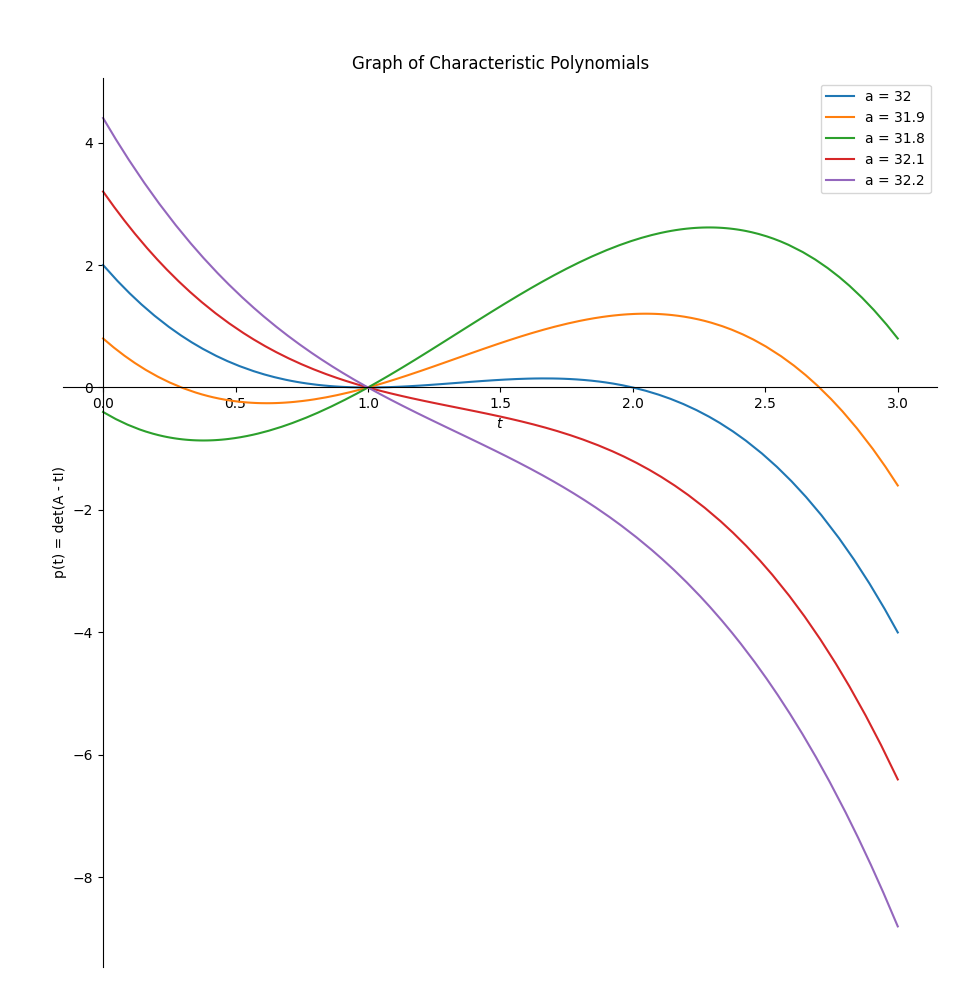
\includegraphics[scale=0.7]{graph.png}}
    \caption{Graph of $p(t) = det(A -tI), 0 \le t \le 3$}
\end{figure}

\newpage

% how does the graph reveal the changes in the eigenvalues as a changes?
The graph shows that as $a$ increases, the eigen values of $A$ move further away from each other. This is because the eigen values of $A$ are the roots of the characteristic polynomial of $A$. As $a$ increases, the roots of the characteristic polynomial move further away from each other.

\section*{Problem 3}

\begin{center}
    Let A = $\begin{bmatrix}
        1 & 0 \\
        6 & -1
    \end{bmatrix}$
\end{center}
Since A is a triangular matrix, the eigen values of A are the diagonal entries of A.

$\therefore$ The eigen values of A are 1 and -1. \\ \\
Finding the eigenvalues of A using $(A - \lambda I)x = 0$.
\begin{center}
    when $\lambda = 1$ \\
    \begin{align*}
        (A - \lambda I)x = 0 \\ \\
        \left(\begin{bmatrix}
            1 & 0 \\
            6 & -1
        \end{bmatrix} - 1 \begin{bmatrix}
            1 & 0 \\
            0 & 1
        \end{bmatrix}\right)x = \begin{bmatrix}
            0 \\
            0
        \end{bmatrix} \\ \\
        \begin{bmatrix}
            0 & 0 \\
            6 & -2
        \end{bmatrix}x = \begin{bmatrix}
            0 \\
            0
        \end{bmatrix} \\ \\
        \text{Augmenting the matrix with } \boldsymbol{0}, \\ \\
        \implies \begin{bmatrix}
            0 & 0 & 0 \\
            6 & -2 & 0
        \end{bmatrix} \\ \\
        \text{Interchange } R_1 \text{ and } R_2 \\ \\
        \begin{bmatrix}
            6 & -2 & 0 \\
            0 & 0 & 0
        \end{bmatrix}
    \end{align*}

    \newpage

    \[
        R_1 \rightarrow \frac{1}{6}R_1
    \]
    \[
        \begin{bmatrix}
            1 & -\frac{1}{3} & 0 \\
            0 & 0 & 0
        \end{bmatrix}
    \]
\linebreak
    General solution is $\begin{cases}
        x_1 = \frac{1}{3}x_2 \\
        x_2 = x_2
    \end{cases}$

    \[
        \implies x = \begin{bmatrix}
            \frac{1}{3}x_2 \\
            x_2
        \end{bmatrix} = x_2 \begin{bmatrix}
            \frac{1}{3} \\
            1
        \end{bmatrix}
    \]

    $\therefore$ The corresponding eigen vector when $\lambda = 1$ is $\begin{bmatrix}
        \frac{1}{3} \\
        1
    \end{bmatrix}$.

\end{center}

\begin{center}
    When $\lambda = -1$ \\
    \begin{align*}
        \left(\begin{bmatrix}
            1 & 0 \\
            6 & -1
        \end{bmatrix} + 1 \begin{bmatrix}
            1 & 0 \\
            0 & 1
        \end{bmatrix}\right)x = \begin{bmatrix}
            0 \\
            0
        \end{bmatrix} \\ \\
        \begin{bmatrix}
            2 & 0 \\
            6 & 0
        \end{bmatrix}x = \begin{bmatrix}
            0 \\
            0
        \end{bmatrix} \\ \\
        \text{Augmenting the matrix with } \boldsymbol{0}, \\ \\
        \implies \begin{bmatrix}
            2 & 0 & 0 \\
            6 & 0 & 0
        \end{bmatrix} \\ \\
        R_2 \rightarrow -3R_1 + R_2 \\ \\
        \begin{bmatrix}
            2 & 0 & 0 \\
            0 & 0 & 0
        \end{bmatrix} \\ \\
        R_1 \rightarrow \frac{1}{2}R_1 \\ \\
        \begin{bmatrix}
            1 & 0 & 0 \\
            0 & 0 & 0
        \end{bmatrix}
    \end{align*}

    \newpage
    General solution is $\begin{cases}
        x_1 = 0 \\
        x_2 = x_2
    \end{cases}$
    \[
        \implies x = \begin{bmatrix}
            0 \\
            x_2
        \end{bmatrix} = x_2 \begin{bmatrix}
            0 \\
            1
        \end{bmatrix}
    \]
\end{center}

To diagonalise the matrix, we need $D$ and $P$ such that $A = PDP^{-1}$.

\[
    D = \begin{bmatrix}
        1 & 0 \\
        0 & -1
    \end{bmatrix} \text{  \&  } P = \begin{bmatrix}
        \frac{1}{3} & 0 \\
        1 & 1
    \end{bmatrix}
\]

\end{document}
